
%%% Local Variables: 
%%% mode: latex
%%% TeX-master: t
%%% End: 

\chapter{资源管理可编程体系结构}
\label{chap:pardarch}

为了保障计算机硬件资源的共享访问性能,本文提出了资源管理可编程体系结构,
通过在硬件上增加资源管理的可编程支持,实现共享硬件资源的可管理共享。
由于计算机内部可以被看作一个内部网络,
通过将网络领域中区分化服务的思路引入计算机体系结构中,
共享硬件资源可以实现对不同应用的区分,
并通过可编程的方式区分处理来自不同应用的请求,实现可管理的共享。
通过这种可管理的共享,可以消除由于共享硬件资源竞争所引入的应用之间的干扰,
使得共享硬件资源的多个应用的性能是可预测且可管理的。
在这样的体系结构下,可以很容易的在同一台服务器上部署更多应用来提高资源利用率,
同时通过对共享硬件资源的可管理共享来保障关键应用的服务质量。
本文设计了一种资源管理可编程体系结构的实现PARD
(Programmable Architecture for Resourcing-on-Demand)\cite{pard2015},
本章将总览PARD架构及其关键特性,
并分析如何利用PARD所提供的特性解决应用服务质量与资源利用率相冲突的问题。


\section{PARD体系结构}

PARD是在传统服务器体系结构的基础上进行功能扩展,
实现硬件资源可管理与区分化服务的计算机体系结构实现。
可以从用户、管理员和体系结构三个视角理解PARD体系结构(如图\ref{fig:pard-views}):
从用户的视角,PARD是一个可以划分为多个子机器的服务器,
各个子机器相互独立,可以运行各自的操作系统,而且对用户来说子机器的执行性能是稳定可预测的;
%不同用户的子机器之间不会存在干扰,用户可根据自己的需求对资源的使用情况进行约定,
%如Cache占用、访存带宽等,
从管理员的视角,PARD是一台具有硬件资源细粒度管理能力的服务器,
管理员可通过服务器上配置的资源管理模块(Platform Resource Manager,PRM)对硬件资源进行管理,
包括硬件资源的划分与监控,并可根据用户需求对资源分配进行调整;
从体系结构的视角,PARD将网络的概念引入到计算机体系结构中,
在体系结构内实现了应用区分,为共享硬件部件增加可编程能力,并实现计算机内统一的资源管理。
基于用户(应用)的\textbf{区分化服务}以及细粒度的硬件\textbf{资源管理}是
PARD区别于传统计算机体系结构的两个主要特征。

%DiffServ
区分化服务(Differentiated Services)起源于计算机网络领域,用于实现网络中的优先级模型,
其核心是在网络包上标记其所属应用的类型,如XXX,XXX,VoIP等,
交换机、路由器等网络设备根据该标记对不同的网络包执行不同的策略来满足其性能需求。
PARD借用了网络中区分化服务的概念,通过为不同应用(用户)分配标签,
将该标签标记到计算机中所有由该应用发出的请求包中,
硬件部件根据该标签对来自不同应用的请求进行区分处理。
通过标签的方式将应用的需求(如性能、或安全性等)传递到硬件,

%资源管理
在计算机领域,资源管理是指控制多少系统资源被分配给特定的应用,
资源的分配与调度是需要完成的首要任务,
即解决“分配多少资源”以及“何时使用资源”的问题。
%其目标是为应用分配足够的资源来完成其任务。
传统计算机体系结构中,硬件并没有提供或只提供了很少的资源管理支持,
硬件资源无条件的暴露给软件,由软件实现对硬件资源的共享管理。
在大部分系统中,操作系统或虚拟化层承担着这一任务,
实现了对部分硬件资源如处理器核、内存容量、网络带宽、I/O设备等的管理。
使用软件进行资源管理会在系统中引入额外的开销\cite{},同时也增加了软件实现的复杂度。
现有的硬件机制已经能够实现将资源管理的功能下放到硬件层次,
相关工作如NoHype\cite{}实现了无需软件干预的资源管理。
在PARD中,区分化服务机制的存在使得硬件能够区分出不同的应用,
在硬件层次实现细粒度的资源管理更为便利。

%软件实现资源管理开销大、将部分功能off-load到硬件可以简化软件实现
%在相关工作中可以列一下软件实现管理的代码开销和性能开销

%PARD所提出的细粒度硬件资源管理将更多的与应用性能相关的硬件资源也纳入到管理域中

资源管理的另一个任务是控制异常应用对共享资源的访问行为,
防止失控的异常访问对其它正常应用的运行造成影响。
在当前虚拟化与云计算场景下,越来越多的应用被运行在共享服务器上,
对异常应用的控制显得愈发重要。
现有体系结构实现中,包含了对处理器核、内存容量、I/O设备的隔离,
但另一部分与应用性能密切相关的共享硬件资源,如共享缓存、总线、访存带宽等,
并没有提供足够的管理支持。
在PARD体系结构下,可管理的硬件资源范围被扩展,
以上这些目前尚未被管理的部件也纳入到需要被管理的共享硬件资源中,
通过PARD所增加的体系结构上的支持,实现对计算机内所有共享硬件资源的管理。


\begin{figure}[t]
  \centering
  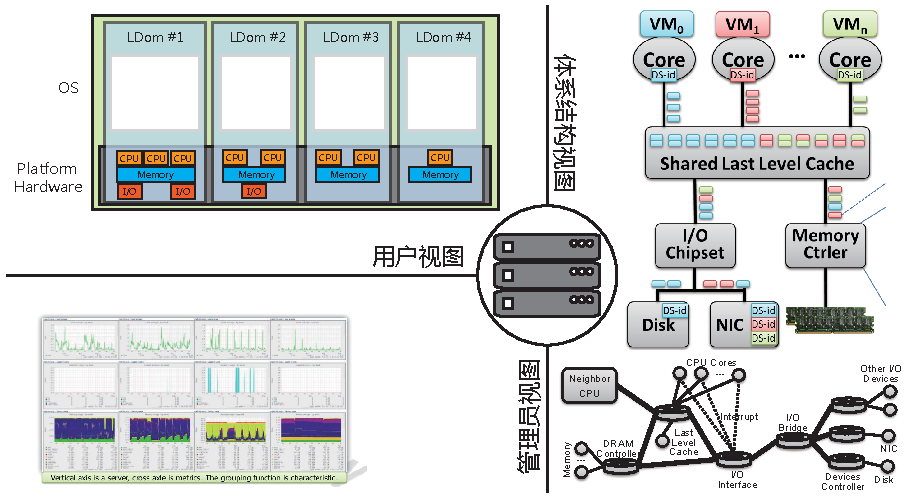
\includegraphics[width=\textwidth]{arch/pard-views.pdf}
  \caption{不同视角下的PARD体系结构}
  \label{fig:pard-views}
\end{figure}

在多应用混合这种共享场景中,隔离性和可管理性是服务器体系结构设计时需要考虑的重要问题。
\textbf{隔离性}是指要让运行在共享环境中的应用无法感知到其它应用的存在,
就像它正在运行在独占的计算机中一样,这其中包含两个层次的概念:
一是资源隔离,即应用独占分配给它的资源;
二是性能隔离,使得应用的性能不会被其它应用所干扰。
现有的软件方案(如多进程、容器、虚拟化)或硬件方案(如LPAR、Logic Domain)
可以很容易实现不同级别的资源隔离,但它们都无法完全实现性能隔离。
首先,在操作系统或虚拟化的软件栈的各个层次中都存在不同程度的共享,
这些共享点在一些特定的场景会产生干扰;
而即使是硬件隔离方案,虽然消除了软件层次的干扰,但在共享硬件资源上的干扰依然存在。
硬件层次的隔离没有发挥应有的效果主要是由于目前的体系结构中并不能识别不同的应用。
\textbf{可管理性}是能够对应用占用的资源进行监控与管理。
由于不同的应用或应用运行的不同阶段,其对资源的需求是不同且不断变化的,
如何获取应用资源需求的变化,以及如何根据这些变化对资源的分配进行调整。

PARD选择了硬件隔离方案,为用户提供逻辑域的抽象以实现资源隔离,
通过使用标签的方式将服务器划分为不同的地址空间,以实现性能隔离;
在各个硬件部件上增加了控制平面与可编程功能,实现共享资源管理;
通过节点内全局的资源管理,实现资源按需分配与动态调整。


\subsection{逻辑域抽象}

当前数据中心软件大都采用分层或基于服务的架构,软件的功能被逐步细化到应用,
单个应用所负载的任务十分简单,无法充分利用服务器全部的硬件资源,
采用某种抽象将多个应用整合到同一台服务器是现在主流的方式。
多应用共享服务器有多种不同的模式,对应的应用也存在不同类型的抽象,如多进程\cite{}、
容器\cite{}、虚拟机\cite{}、逻辑域\cite{}或逻辑分区\cite{}等,
PARD选取与了逻辑域类似的方案,将一个物理系统划分为多个相互独立的虚拟系统,
这些虚拟系统即为逻辑域。
每个逻辑域只包含物理系统部分硬件资源(如内存、处理器、I/O),不同逻辑域之间相互隔离,
它们运行自己的操作系统,拥有独立的资源与标识。

逻辑相关或数据交换较为频繁的应用通常会被部署到相同的物理服务器,
这些逻辑域组成一个应用组,在应用组内可以可建立任意拓扑的链路,用于组内逻辑域间的通信。

资源分配是可编程的,数据通路拓扑是可编程的,除此之外,性能也是可编程的。
除那些必须被分配的资源外,一些共享的与性能相关的资源在PARD中也可以按逻辑域或应用组进行分配。

使用逻辑域抽象,可以很容易的将现有的软件架构映射到PARD中,以两种典型的应用为例:
分布式RPC与网络功能虚拟化(NFV)、MapReduce计算框架。
分布式RPC分为框架与服务两部分,


\subsection{应用示例:用户与管理员视角}

本节将从用户和管理员的视角,给出PARD在共享数据中心场景中的应用,
介绍PARD的关键特性,以及如何使用PARD解决硬件资源共享带来的干扰问题,
图\ref{fig:pard-example}为该示例的流程。

\begin{figure}[tb]
  \centering
  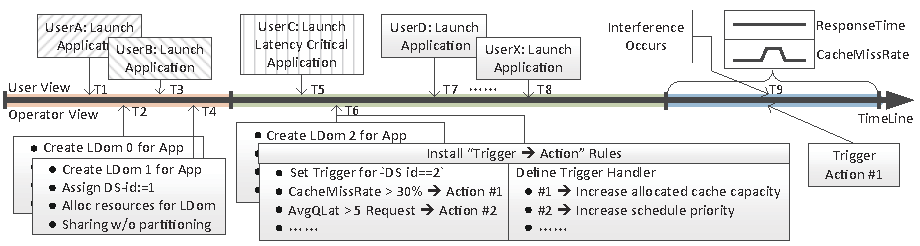
\includegraphics{arch/pard-example.pdf}
  \caption{PARD示例}
  \label{fig:pard-example}
\end{figure}

1. 在T1和T3时间,用户A和用户B分别希望在服务器上运行应用,
他们将自己的资源需求发送到管理员,管理员在收到请求后,
决定将两个用户的应用运行在同一台PARD服务器上。
在真实的场景中,用户与管理员并不会直接操作服务器,
而是通过如mesos\cite{}、OpenStack\cite{}等集群管理系统使用服务器资源。
这里为了简化描述,将集群管理系统这一层移除,让用户与管理员直接操作服务器。

2. 管理员在T2和T4时刻分别处理用户的请求,并通过服务器的PRM接口将资源需求发送到服务器,
交由运行在PRM中的固件对请求进行处理,并分配资源。
以用户B为例,PRM首先为其创建一个逻辑域(LDom),并根据需要为其分配资源,
该逻辑域的编号为“1”(后续使用LDom1表示该逻辑域)。
由于LDom1是一个普通优先级的应用,PRM为其分配了默认的资源使用策略:
与其它逻辑域共享末级缓存、内存、I/O等硬件资源。
在将这些策略编程到各个设备的控制平面后,PRM完成对LDom1的初始化,并在其中启动操作系统。

3. 在T5时刻,用户C希望执行一个高优先级、延迟敏感型的应用,并通过管理员将请求发送到PRM。
在T6时刻,PRM创建了逻辑域LDom2,并为其分配了高优先级的资源分配策略,
在完成LDom2的初始化后,将用户C的应用部署在该逻辑域中。

4. 在T7和T8时刻,更多的用户将资源需求提交到服务器,服务器的资源利用率持续上升。

5. 在T9时刻,由于服务器内运行的应用在共享末级缓存中产生了严重的干扰,
用户C应用的缓存缺失率急剧上升(>30\%)。
在传统的服务器中,如此高的缓存缺失率会造成应用性能的严重下降,
响应时间出现明显的长尾。而在PARD服务器中,用户C的缓存缺失率上升达到30\%时,
末级缓存会向PRM发送该事件的事件通知,运行在PRM中的固件检测到该事件通知,
执行该事件对应的动作脚本,实现资源的重新分配。
在本例中,该事件的动作脚本将为用户C分配更多的末级缓存容量,以缓解其缺失率更高的问题。
通过以上动作,使得在PARD服务器中用户C应用的性能(响应时间)没有受到严重的影响。


\subsection{体系结构视角}

从体系结构的视角(图\ref{fig:pard-arch-detail}),
PARD在传统的体系结构之上增加了额外的资源管理系统,将业务处理与资源管理两项工作分离,
用户只工作在业务系统上,而管理员仅在管理系统上即可实现用户资源使用的监控与管理。

\begin{figure}[tb]
  \centering
  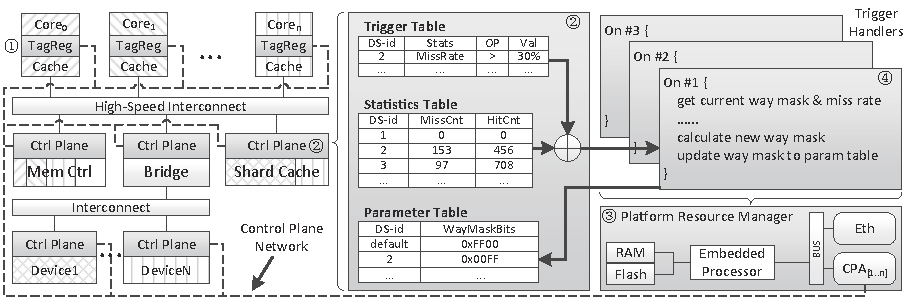
\includegraphics[width=\textwidth]{arch/pard-arch-detail.pdf}
  \caption[PARD体系结构]{PARD体系结构,图中灰色方框为PARD在现有体系结构中所增加的组件}
  \label{fig:pard-arch-detail}
\end{figure}

PARD体系结构基于“计算机内部是一个网络”这样一个观察,
为了让“内部网络”中的设备(共享硬件资源)能够识别出不同应用的请求,
PARD在所有请求源(如处理器核和具有DMA功能的I/O设备)上增加标签寄存器,
该寄存器的值用于标记网络中所有的请求包,如cache请求、访存请求、DMA请求或中断请求。
在当前的PARD实现中,使用逻辑域作为标签粒度,实际上该粒度可以继续细分,
实现容器级、进程级、线程级甚至代码段级别的标签。

由于“内部网络”中的每一个请求都包含了其所属应用的标签,
PARD在共享硬件资源上引入了控制平面的概念,利用应用标签实现资源管理与区分化服务。
控制平面采用其于表的设计,其中包含三个由应用标签索引的控制表:
参数表(parameter table),用于记录资源分配策略;
状态表(statistics table),用于统计资源使用情况;
触发表(trigger table),用于保存性能触发规则。
这些控制表实现了共享资源管理的编程接口,
控制平面根据控制表中的信息对接收到的请求采取不同的动作。
当收到新的请求后,控制平面首先查询参数表,获得该请求的资源分配策略,对请求进行预处理,
如资源分配、请求调度、地址变换、数据预处理等,
之后将预处理后的请求发送到硬件完成操作,在完成操作后更新状态表,同时检查触发表以匹配触发规则,
如果某一触发规则被满足时,通过中断接口向外发送该触发事件。

PARD使用独立的集中式平台资源管理模块(PRM)管理节点内所有的共享硬件资源,
具体包括对控制表的配置和查询,以及接收并处理控制平面发出的触发事件。
与目前服务器普遍配置的IPMI/BMC模块类似,PRM也是基于SoC系统实现,
其中包含处理器、内存、flash存储、以太网接口等。
除此之外,PRM中还包含一个控制平面适配器(CPA),
该适配器连接到系统中所有的控制平面,组成控制平面网络,
PRM通过该网络实现对控制平面的操作,完成硬件资源管理的功能。
PRM上运行基于linux的固件,将全部控制平面抽象为文件树的形式,
管理员可以集中管理所有的控制平面,在各个硬件上为不同的应用制定策略和性能触发规则。

% TODO: add more information


\subsection{关键特性}

在上面两节中,分别从用户、管理员与体系结构视角对PARD的关键特性进行了描述,
本节将对这些特性进行总结,并简要介绍其实现原理,具体的内容将在后续章节进行详细分析。

% 关键技术点
\textbf{标签化地址空间}\ 传统计算机架构使用单一地址空间,虽然虚拟内存与扩展页表机制
为不同的应用或虚拟机分配独立的逻辑地址空间,但它们还是共享一个物理地址空间。
这种单一地址空间的设计,使得共享的硬件部件不能识别出来自不同应用的请求,
造成应用之间由于竞争硬件资源而产生相互之间的干扰,影响应用的性能。
标签化地址空间是指让计算内所有的请求都携带应用的标签信息,
让共享的硬件部件能够识别出来自不同应用的请求,以实现应用之间的区分化服务。
标签粒度有多种选择,可根据实际的应用需求使用虚拟机、容器、进程、线程
或是一个代码段作为标签。
在现有体系结构上实现标签化地址空间主要需要三个方面的修改:
%第一方面,加寄存器
首先,需要在请求的发起端(如处理器核或带有DMA的I/O设备)增加一个标签寄存器,
用以记录当前应用的标签,并在请求产生后将标签附加到请求上;
%扩展数据通路,传播标签
之后需要在计算机内的数据通路中传播请求的标签,
这些数据通路包括片上网络、处理器之间的互连总线(如QPI或HT)、
I/O总线(如PCI-E)等,目前的体系结构实现中这些总线都使用基于包的总线协议,
因此可以很容易的扩展请求包,将应用标签附加到总线上;
%修改不支持标签传播的硬件,如Cache
第三,修改数据通路上一些不能支持应用标签传播的硬件部件,
使其能够将应用标签正确的传播到下一级通路,
以共享末级缓存为例,对于使用WriteBack策略的共享末级缓存,
由于缓存替换所引起的写回操作,被替换的数据与造成替换的请求并非属于同一个应用,
因此需要在缓存的TagArrary中记录数据所属的应用标签,
在发生缓存替换时,被写回的数据需要附加上TagArray中记录的应用标签,
而不是引起缓存替换的请求所附带的应用标签。
本文将在第\ref{chap:labeladdrspace}章详细讨论在现有体系结构下如何实现标签化地址空间。


%简单说就是加控制平面做管理,数据平面加处理器实现可编程
\textbf{可管理的硬件资源共享}\ 在通过标签化地址空间实现应用区分后,需要对硬件资源的共享访问进行管理。
在现有的体系结构实现下,已经存在一些硬件支持共享管理,
如处理器可通过时间片调度的方式对共享行为进行管理,
Intel在其最新的Xeon E5v3系列处理器中增加了对Cache的容量划分的支持\cite{intel-cat},
可以通过其增加的配置寄存器管理不同应用允许使用的缓存容量。
但除些之外,其它一些重要的共享硬件资源,如内存控制器、I/O等,并不支持对应用共享访问进行管理。
例如,现有的体系结构实现下,无法实现调整某一应用所能够使用的访存带宽、访存优先级或I/O带宽等。
本文提出一种硬件资源共享管理的方法,让计算机内所有重要的共享硬件都支持共享管理,
同时为上层管理员提供一个统一的管理接口。
该方法来源于软件定义网络(SDN)中所提出的控制平面与数据平面的概念,
在SDN中,通过将网络设备划分为控制平面与数据平面,使用控制平面进行管理,数据平面进行转发,
以实现灵活的网络管理。
由于计算机可以被看作是一个网络,与SDN的方法类似,
通过修改硬件的“数据平面”,为其增加可编程能力,实现对应用进行区分处理的功能,
并为硬件部件中增加控制平面,为上层提供统一的资源管理接口,
管理数据平面可编程机制所提供的共享管理特性。
其中控制平面使用基于表的方式,为上层提供管理接口,而数据平面中使用可编程处理器的方式为硬件提供灵活的管理功能,
本文第\ref{chap:hwresman}章将对PARD所提供的硬件资源共享管理机制进行详细讨论。


% 资源监控 + Trigger=>Action反馈 + 全局资源调节
\textbf{资源按需分配}\ 集中式的资源监控,资源全局调节,Trigger=>Action的反馈调节机制。


本文第\ref{chap:hwresman}章将对资源监控与反馈调节机制进行分析,资源的全局管理将在第\ref{chap:global}章进行讨论。


\section{PARD服务器操作}

本节介绍PARD服务器基本操作流程,包括逻辑域创建、资源调整、以及性能监控与反馈。
首先我们定义一台PARD服务器,本节后续内容将以该PARD服务器为实例,
其主要配置如下:

8个处理器核,每个处理器核中包含私有L1 I-Cache和D-Cache;

共享16MB的L2 Cache,使用24路组相联映射;

共享内存控制器,内存容量为8GB;

共享I/O子系统,包含8个SATA硬盘和4个千兆以太网卡。

该服务器共享硬件资源(处理器核、L2 Cache、内存控制器、I/O子系统)都实现了
上节所述的控制平面,其控制表项目以及实现的功能如表\ref{}所示。
所有控制平面都通过控制平面网络连接到PRM,PRM上运行用于资源管理的固件。

与服务器中的IPMI/BMC模块类似,PRM是一个嵌入式的SoC系统,用于管理服务器内所有的资源。
当服务器加电启动后,PRM首先启动,并通过控制平面网络获取服务器的硬件资源信息,
后续管理员直接与PRM交互,将PARD服务器配置为多个逻辑域,运行用户的应用。
管理员可以为每个应用设定其监控条件,当某一硬件控制平面发现监控条件满足时,
则通过PRM通知上层管理架构,管理员可以通过PRM对不同应用的硬件资源使用进行管理。
本节后续将从逻辑域的创建、监控条件设定、参数调整三个方面介绍PARD服务器操作。

\subsection{逻辑域创建}

PARD服务器使用逻辑域抽象为用户提供服务,每个逻辑域都是PARD服务器硬件资源的子集,
可直接在其中启动操作系统。不同的逻辑逻辑域独占部分资源,如处理器核、内存、I/O设备;
另一些硬件资源在不同逻辑域中共享,如L2 Cache。
当PRM收到逻辑域的创建请求后,PRM首先确认当前服务器是否有足够的资源满足逻辑域的需求,
如果满足,则为其分配一个本地唯一的逻辑域标识,
之后在各个硬件资源的控制平面中为该逻辑域分配所需的资源。
例如,用户创建的逻辑域需要2个处理器核、2GB内存、一个硬盘和一个网卡,
PRM在确认本地资源充足后,为其分配逻辑域标识LDom\#1,后续的创建流程如下:

(1)查询处理器核的控制平面,找到两个空闲的处理器核,并向其标签寄存器写入LDom\#1,
这两个处理器核后续发出的请求中将都包含该逻辑域标签。

(2)在L2 Cache控制平面中增加LDom\#1的控制表项,由于该用户在创建逻辑域时并没有对
Cache指定特殊需求,因此为其分配默认的替换策略掩码,与其他用户共享L2 Cache。

(3)PRM查询内存地址分配,找到空闲的2GB内存空间,
在内存控制器控制平面中建立逻辑域LDom\#1的控制表项,
将查询到的2GB空闲内存的地址写入控制表项,保存逻辑域与内存地址的关联,
内存控制器在收到后续带有LDom\#1标签的访存请求后,会将查询地址映射信息,
对访存地址进行映射,使得内存控制器对来自不同逻辑域的请求进行区分处理。

(4)PRM为逻辑域分配磁盘和网卡,通过I/O控制平面将两个设备的标签寄存器设置为LDom\#1。
这两个设备对内存的DMA请求中都包含该标签,保证其能够访问到逻辑域的内存地址空间;
当前大部分的PCI-E设备都使用MSI方法产生中断,而MSI的本质是对特殊地址的访存请求,
该请求中已经包含了逻辑域标签,因此中断请求能够被正确的发送到分配给该逻辑域的处理器核。

(5)PRM查询这两个设备的物理地址(PA)和所需的I/O地址空间长度,
在逻辑域的地址空间中为这两个设备分配地址(LA),
通过I/O控制平面将分配的PA与LA记录到LDom\#1的控制表项。

在资源分配完成后,PRM通过处理器控制平面,将两个处理器核复位,
之后并选择一个处理器核做为BP,令其开始执行BIOS代码,并启动操作系统。
由于不同的逻辑域使用不同的标识,在整个计算机的数据通路中都能够根据该标识对逻辑域实现区分,
实现逻辑域之间的资源隔离。

在创建逻辑域时,同时还可以指定其性能参数,如Cache替换策略掩码、访存调度优先级、
I/O带宽等,各个硬件部分根据其控制平面中指定的性能参数实现对不同逻辑域的区分化服务。


\subsection{资源调整}

用户的应用在运行时对硬件资源的需求会发生变化,PARD提供了运行时调整硬件资源分配的方法,
允许用户根据需求在运行时对逻辑域的资源分配进行调整,以满足应用的需求。
硬件资源包括可透明调整的资源,如Cache容量、访存带宽等;
也包括需要操作系统支持的资源,如处理器核、内存容量、I/O设备。




\subsection{性能监控与反馈}

性能监控与反馈主要得益于控制平面的设计,通过在硬件上增加控制平面,对请求进行处理,
可以获得不同的应用的状态。如Cache缺失率、访存延迟等。
并通过一个可编程的触发逻辑,当特定事件发生后,将消息通过统一的控制平面网络,
发送到集中式的资源管理模块PRM,由PRM对资源分配进行调整。

在第\ref{chap:}中将对控制平面的设计,以及资源监控进行详细的分析。


\section{服务质量与资源利用率}


\section{小结}

